\documentclass{beamer}

% Beamer style
%\usetheme[secheader]{Madrid}
\usetheme{CambridgeUS}
\usecolortheme[rgb={0.65,0.15,0.25}]{structure}
%\usefonttheme[onlymath]{serif}
\beamertemplatenavigationsymbolsempty
%\AtBeginSubsection

% Packages
%\usepackage[french]{babel}
\usepackage[latin1]{inputenc}
\usepackage{color}
%\usepackage{dsfont, stmaryrd}
\usepackage{amsmath, amsfonts, amssymb}
\usepackage{epsfig}
\usepackage{url}
\usepackage{/home/robin/LATEX/astats}
%\usepackage[all]{xy}
\usepackage{graphicx}

% Commands
\definecolor{darkred}{rgb}{0.65,0.15,0.25}
\newcommand{\emphase}[1]{\textcolor{darkred}{#1}}
%\newcommand{\emphase}[1]{{#1}}
\newcommand{\paragraph}[1]{\textcolor{darkred}{#1}}
\newcommand{\refer}[1]{{{\textcolor{blue}{{\cite{#1}}}}}}
\newcommand{\Refer}[1]{{{\textcolor{blue}{{\sl #1}}}}}
\newcommand{\newblock}{}

% Symbols
\newcommand{\Abf}{{\bf A}}
\newcommand{\Beta}{\text{B}}
\newcommand{\Bcal}{\mathcal{B}}
\newcommand{\BIC}{\text{BIC}}
\newcommand{\Ccal}{\mathcal{C}}
\newcommand{\dd}{\text{~d}}
\newcommand{\dbf}{{\bf d}}
\newcommand{\Dcal}{\mathcal{D}}
\newcommand{\Esp}{\mathbb{E}}
\newcommand{\Ebf}{{\bf E}}
\newcommand{\Ecal}{\mathcal{E}}
\newcommand{\Gcal}{\mathcal{G}}
\newcommand{\Gam}{\mathcal{G}\text{am}}
\newcommand{\Ibb}{\mathbb{I}}
\newcommand{\Ibf}{{\bf I}}
\newcommand{\ICL}{\text{ICL}}
\newcommand{\Cov}{\mathbb{C}\text{ov}}
\newcommand{\Corr}{\mathbb{C}\text{orr}}
\newcommand{\Var}{\mathbb{V}}
\newcommand{\Vsf}{\mathsf{V}}
\newcommand{\pen}{\text{pen}}
\newcommand{\Fcal}{\mathcal{F}}
\newcommand{\Hbf}{{\bf H}}
\newcommand{\Hcal}{\mathcal{H}}
\newcommand{\Jcal}{\mathcal{J}}
\newcommand{\Kbf}{{\bf K}}
\newcommand{\Lcal}{\mathcal{L}}
\newcommand{\Mcal}{\mathcal{M}}
\newcommand{\mbf}{{\bf m}}
\newcommand{\mum}{\mu(\mbf)}
\newcommand{\Ncal}{\mathcal{N}}
\newcommand{\Nbf}{{\bf N}}
\newcommand{\Nm}{N(\mbf)}
\newcommand{\Ocal}{\mathcal{O}}
\newcommand{\Obf}{{\bf 0}}
\newcommand{\Omegas}{\underset{s}{\Omega}}
\newcommand{\Pbf}{{\bf P}}
\newcommand{\Pcal}{\mathcal{P}}
\newcommand{\Qcal}{\mathcal{Q}}
\newcommand{\Rbb}{\mathbb{R}}
\newcommand{\Rcal}{\mathcal{R}}
\newcommand{\sbf}{{\bf s}}
\newcommand{\Sbf}{{\bf S}}
\newcommand{\Scal}{\mathcal{S}}
\newcommand{\Ucal}{\mathcal{U}}
\newcommand{\Vcal}{\mathcal{V}}
\newcommand{\Tbf}{{\bf T}}
\newcommand{\ubf}{{u}}
\newcommand{\Ubf}{{U}}
\newcommand{\Wbf}{{W}}
\newcommand{\xbf}{{x}}
\newcommand{\Xbf}{{X}}
\newcommand{\ybf}{{y}}
\newcommand{\Ybf}{{Y}}
\newcommand{\zbf}{{z}}
\newcommand{\Zbf}{{Z}}
\newcommand{\betabf}{\text{\mathversion{bold}{$\beta$}}}
\newcommand{\pibf}{\text{\mathversion{bold}{$\pi$}}}
\newcommand{\phibf}{\text{\mathversion{bold}{$\phi$}}}
\newcommand{\Sigmabf}{\text{\mathversion{bold}{$\Sigma$}}}
\newcommand{\gammabf}{\text{\mathversion{bold}{$\gamma$}}}
\newcommand{\mubf}{\text{\mathversion{bold}{$\mu$}}}
\newcommand{\nubf}{\text{\mathversion{bold}{$\nu$}}}
\newcommand{\Thetabf}{{\Theta}}
\newcommand{\thetabf}{{\theta}}
\newcommand{\BP}{\text{BP}}
\newcommand{\EM}{\text{EM}}
\newcommand{\VEM}{\text{VEM}}
\newcommand{\VBEM}{\text{VBEM}}
\newcommand{\cst}{\text{cst}}
\newcommand{\obs}{\text{obs}}
\newcommand{\ra}{\emphase{\mathversion{bold}{$\rightarrow$}~}}
\newcommand{\QZ}{Q_{\Zbf}}
\newcommand{\Qt}{Q_{\thetabf}}
%\newcommand{\transp}{\text{{\tiny $\top$}}}
\newcommand{\transp}{\text{{\tiny \mathversion{bold}{$\top$}}}}

% Directory
\newcommand{\figmixt}{/home/robin/ENSEIGN/COURS/MELANGE}
\newcommand{\figbma}{/home/robin/RECHERCHE/RUPTURES/MELANGE/Exemples/Grippe}
\newcommand{\fignet}{../FIGURES}
\newcommand{\figeco}{/home/robin/RECHERCHE/ECOLOGIE/EXPOSES/FIGURES}
%\newcommand{\figmotif}{/home/robin/RECHERCHE/RESEAUX/Motifs/FIGURES}


%--------------------------------------------------------------------
%--------------------------------------------------------------------

%--------------------------------------------------------------------
%--------------------------------------------------------------------
\begin{document}
%--------------------------------------------------------------------
%--------------------------------------------------------------------

%--------------------------------------------------------------------
\title[Structure in interaction networks]{Deciphering hidden structure in interaction networks}   

\author[S. Robin]{\emphase{A. Channarond}, S. Robin}

\institute[INRA / AgroParisTech]{INRA / AgroParisTech \\
  \vspace{-1cm}
  \begin{tabular}{ccccc}
    
\includegraphics[width=2.5cm]{\fignet/LogoINRA-Couleur} & 
    \hspace{.5cm} &
    
\includegraphics[width=3.75cm]{\fignet/logagroptechsolo} & 
    \hspace{.5cm} &
    
\includegraphics[width=2.5cm]{\fignet/logo-ssb}
    \\ 
  \end{tabular} \\
  \bigskip
  }

\date[R-Syst'13]{R-Syst Meeting, November 2013, Orl�ans}

%--------------------------------------------------------------------
%--------------------------------------------------------------------
\maketitle
%--------------------------------------------------------------------

%--------------------------------------------------------------------
%--------------------------------------------------------------------
\section{Heterogeneity in interaction networks}
\frame{\frametitle{Heterogeneity in interaction networks}}
%--------------------------------------------------------------------

%--------------------------------------------------------------------
\frame{\frametitle{Understanding network structure}

  Networks describe interactions between entities. \\
  ~\\
  Observed networks display heterogeneous topologies, that one would like to decipher and better understand. \\
  ~\\

  \pause
    \begin{tabular}{ll}
    %\hspace{-.5cm}
    \begin{tabular}{p{.5\textwidth}}
      \paragraph{Dolphine social network.} \\
      %\epsfig{file=../Figures/NeG04-Fig11.ps, clip=, width=.5\textwidth}
      \includegraphics[width=.4\textwidth]{../FIGURES/NeG04-Fig11} \\
      \refer{NeG04}
    \end{tabular}
    & 
    \hspace{-.5cm}
    \begin{tabular}{p{.5\textwidth}}
      \paragraph{Hyperlink network.} \\
      \includegraphics[width=.4\textwidth]{../FIGURES/NeG04-Fig13} 
    \end{tabular} 
  \end{tabular} 
  }

%--------------------------------------------------------------------
\frame{\frametitle{An ecological network}

  \hspace{-.1\textwidth}
  \begin{tabular}{cc}
    \begin{tabular}{c}
      {Tree network} \\
      %\epsfig{file=../Figures/NeG04-Fig11.ps, clip=, width=.5\textwidth}
      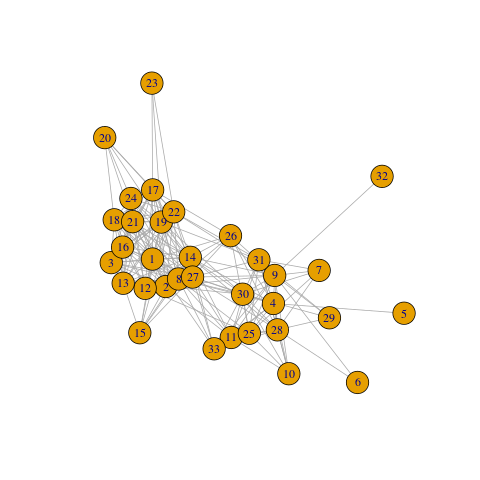
\includegraphics[width=.5\textwidth]{../FIGURES/TreeNetwork-t4} 
    \end{tabular}
    & 
    \hspace{-.1\textwidth}
    \begin{tabular}{c}
      {Fungi network} \\
      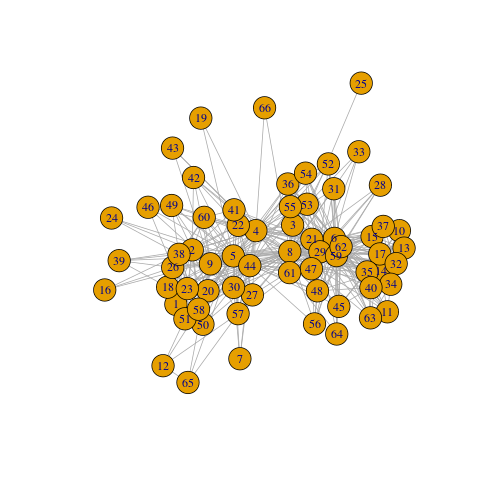
\includegraphics[width=.5\textwidth]{../FIGURES/FungiNetwork-t3} 
    \end{tabular} 
  \end{tabular} \\
  \refer{VPD08}, \refer{MRV10} 
  }

%--------------------------------------------------------------------
\frame{\frametitle{Modelling network heterogeneity}

  \paragraph{Latent variable models} allow to capture
  the underlying structure of a network.

  \bigskip \bigskip \pause
  \paragraph{Model based approach}, in contrast with, e.g.
  \begin{itemize}
  \item Graph clustering \refer{GiN02}, \refer{New04}; 
  \item Spectral clustering \refer{LBB08}.
  \end{itemize}

  \bigskip \bigskip \pause
  \paragraph{General setting for binary graphs.} \refer{BJR07}: %\pause
  \begin{itemize}
   \item   \emphase{A latent (unobserved) variable $Z_i$} is associated with each node
%   $$
%   \{Z_i\} \text{ iid } \sim \pi 
%   $$
  \item   Edges \emphase{$Y_{ij} = \Ibb\{i \sim j\}$ are independent conditionally} to the $Z_i$'s
%   $$
%   \{Y_{ij}\} \text{ independent } | \{Z_i\}: \Pr\{Y_{ij} = 1\} = \gamma(Z_i, Z_j)
%   $$
  \end{itemize}

  }

%--------------------------------------------------------------------
\subsection*{State space models}
%--------------------------------------------------------------------
\frame{ \frametitle{Latent space models}

  \vspace{-0.1\textheight}
  \begin{tabular}{cc}
    \begin{tabular}{p{.5\textwidth}}
     \onslide+<1->{
	\paragraph{State-space model: principle.}}
	 \begin{itemize}
	   \onslide+<2->{
        \item Consider $n$ nodes ($i = 1..n$); \\ ~ } 
        \onslide+<3->{
        \item $Z_i = $ unobserved characteristic \\
        e.g. a 'position' in a 'latent space' \\ ~} 
        \onslide+<4->{
        \item Edges $\{Y_{ij}\}$ independent given $\{Z_i\}$:
          $$
          \Pr\{Y_{ij} = 1\} = \gamma(Z_i, Z_j)
          $$
          Often:
          $
          \gamma(z, z') = f(d(z, z')).
          $
          }
      \end{itemize}
    \end{tabular}
    & 
%     \hspace{-.1\textheight}
    \begin{tabular}{p{.5\textwidth}}
      \vspace{.2\textheight}
      \begin{overprint}
        \onslide<3>
        \hspace{-.1\textwidth}
        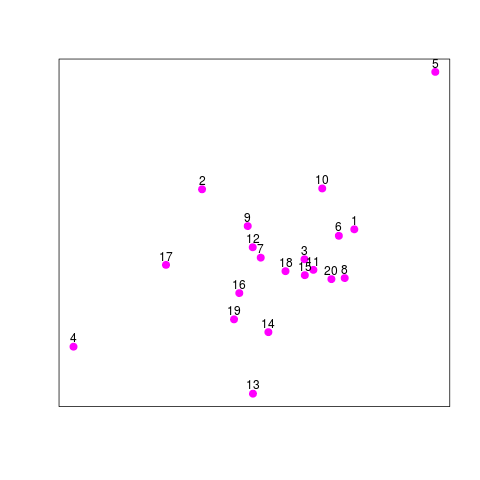
\includegraphics[width=.5\textwidth]{\fignet/FigCLADAG-LPM-Y}    
        \onslide<4>
        \hspace{-.1\textwidth}
        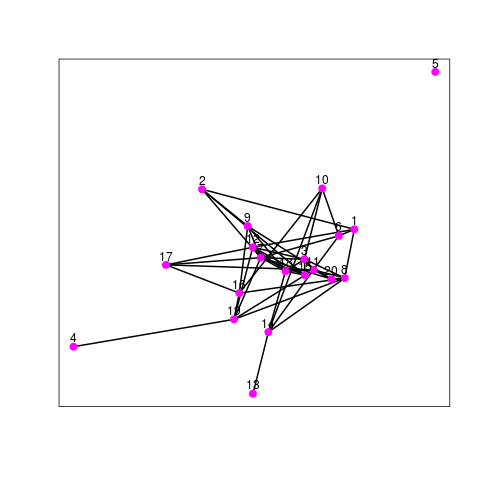
\includegraphics[width=.5\textwidth]{\fignet/FigCLADAG-LPM-XY}    
        \onslide<5>
        \hspace{-.1\textwidth}
        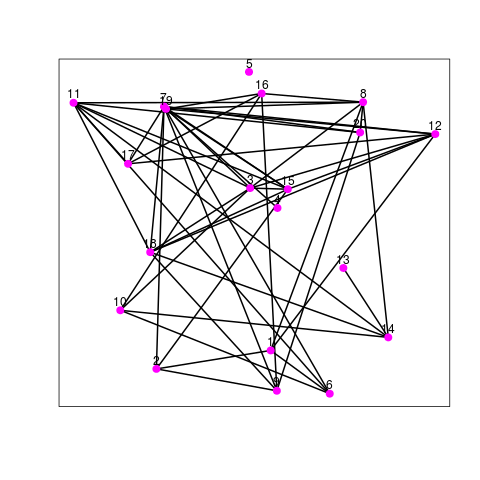
\includegraphics[width=.5\textwidth]{\fignet/FigCLADAG-LPM-X1}    
        \onslide<6>
        \hspace{-.1\textwidth}
        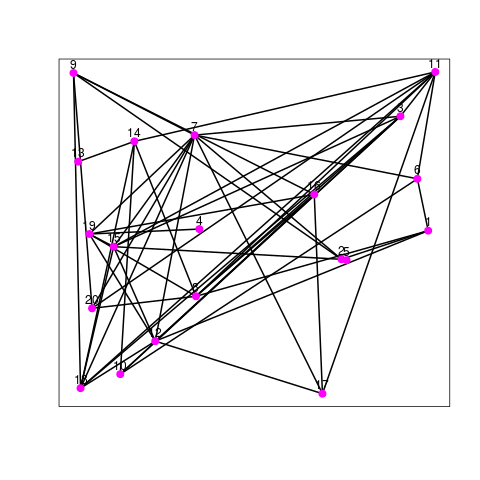
\includegraphics[width=.5\textwidth]{\fignet/FigCLADAG-LPM-X2}    
        \onslide<7>
        \hspace{-.1\textwidth}
%         \vspace{.5\textheight}
%         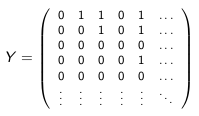
\includegraphics[width=.4\textwidth]{\fignet/FigCLADAG-LPM-adjmat}    
        $
        Y = \left( {\footnotesize
		\begin{array}{cccccc}
		0 & 1 & 1 & 0 & 1 & \dots \\
		  & 0 & 1 & 0 & 1 & \dots \\
		  &   & 0 & 0 & 0 & \dots \\
		  &   &   & 0 & 1 & \dots \\
		  &   &   &   & 0 & \dots \\
		  &   &   &   &   & \ddots  
		\end{array}
        } \right)
        $
      \end{overprint}
      
    \end{tabular}
    
  \end{tabular}

  }

%--------------------------------------------------------------------
\frame{\frametitle{Unclustered vs clustered models}

  \begin{tabular}{cc}
    \begin{tabular}{p{.5\textwidth}}
    {Continuous latent position models.} \\ 
    \onslide+<1->{
    \paragraph{Latent position models} \\ \refer{HRH02}: 
    $$
    Z_i \sim f \text{ \emphase{unimodal}} 
    $$
    $f =$ Gaussian dist. \\ ~ \\
    }
    \onslide+<5->{
    \paragraph{Latent position cluster model}\\ \refer{HRT07}:
    $$
    Z_i \sim f \text{ \emphase{multimodal}}
    $$
    $f =$ Gaussian mixture dist.
    }
    \end{tabular}
    & 
    \begin{tabular}{p{.5\textwidth}}
      \vspace{1cm}
      \begin{overprint}
        \onslide<1>
        \hspace{-.1\textwidth}
        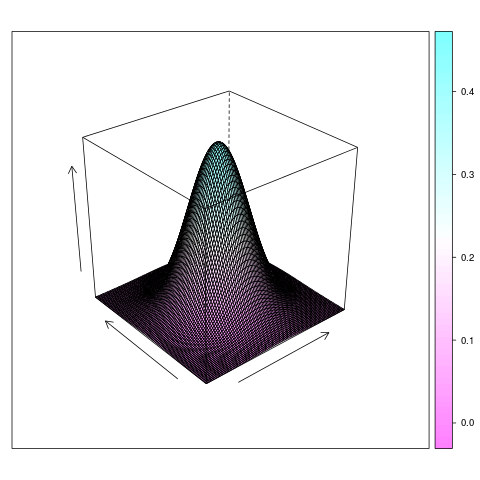
\includegraphics[width=.5\textwidth]{\fignet/FigRSyst-LPM-density}    
        \onslide<2>
        \hspace{-.1\textwidth}
        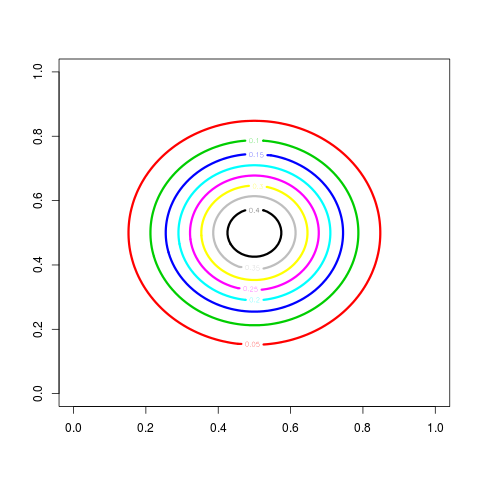
\includegraphics[width=.5\textwidth]{\fignet/FigRSyst-LPM-contour}    
        \onslide<3>
        \hspace{-.1\textwidth}
        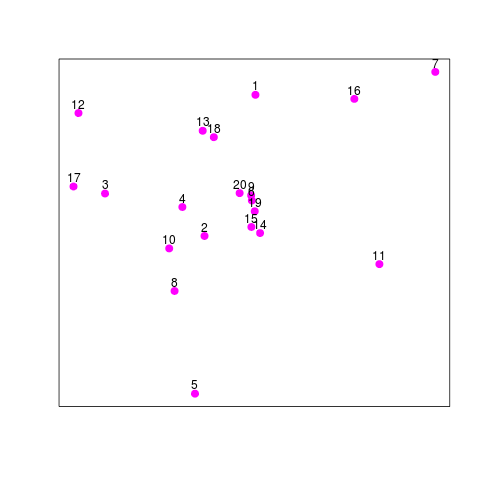
\includegraphics[width=.5\textwidth]{\fignet/FigRSyst-LPM-Y}    
        \onslide<4>
        \hspace{-.1\textwidth}
        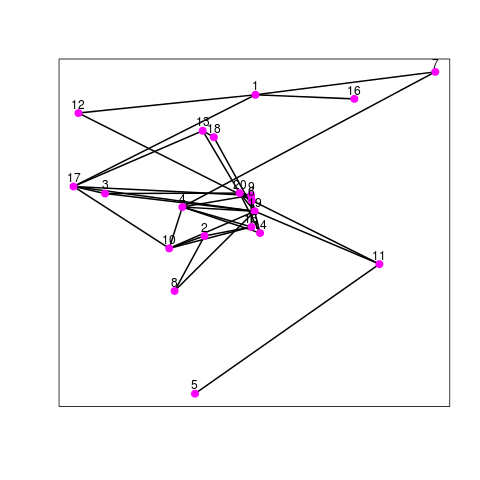
\includegraphics[width=.5\textwidth]{\fignet/FigRSyst-LPM-XY}    
        \onslide<5>
        \hspace{-.1\textwidth}
        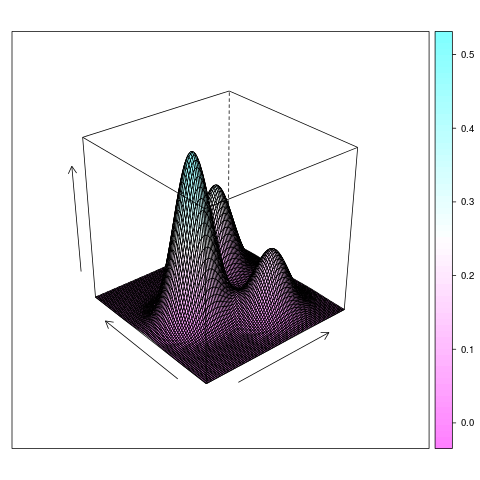
\includegraphics[width=.5\textwidth]{\fignet/FigRSyst-LPCM-density}    
        \onslide<6>
        \hspace{-.1\textwidth}
        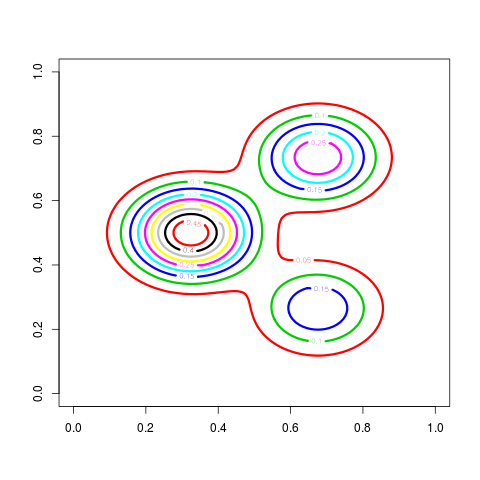
\includegraphics[width=.5\textwidth]{\fignet/FigRSyst-LPCM-contour}    
        \onslide<7>
        \hspace{-.1\textwidth}
        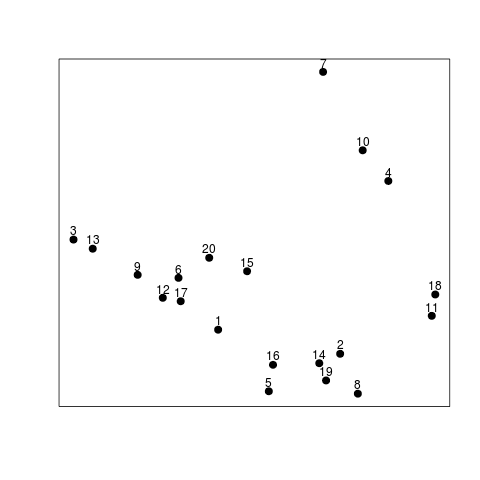
\includegraphics[width=.5\textwidth]{\fignet/FigRSyst-LPCM-Y}    
        \onslide<8>
        \hspace{-.1\textwidth}
        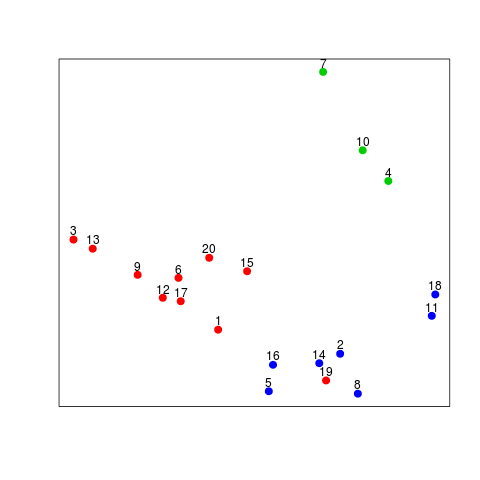
\includegraphics[width=.5\textwidth]{\fignet/FigRSyst-LPCM-YZ}    
        \onslide<9>
        \hspace{-.1\textwidth}
        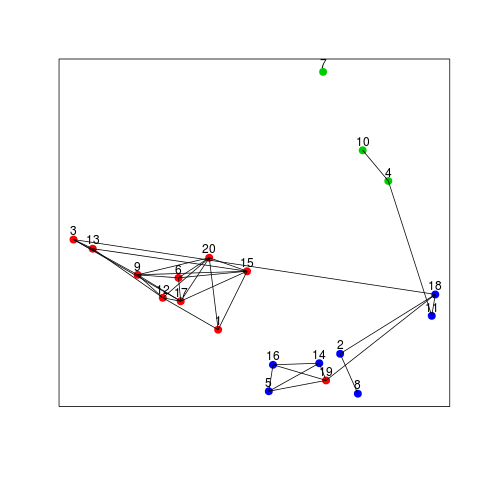
\includegraphics[width=.5\textwidth]{\fignet/FigRSyst-LPCM-XYZ}    
      \end{overprint}
      
    \end{tabular}
    
  \end{tabular}

  }

%--------------------------------------------------------------------
\subsection{Inference in state space models}
%--------------------------------------------------------------------
\frame{\frametitle{Inference in state space models}
  
  \paragraph{General issue.} State space models are part of incomplete data models as
  \begin{itemize}
   \item some variables are observed: the edges $Y_{ij}$
   \item some variables are not observed: the positions $Z_{i}$
  \end{itemize}
  
  \bigskip \pause
  \paragraph{Likelihood-based approach.} Most classical approaches address this issue through iterative algorithm alternating
  \begin{enumerate}
   \item the estimation of the parameters, based on a 'completed' dataset $(Y, \widehat{Z})$
   \item the inference of the missing data $Z$ conditional to $Y$ and the parameters \ra $\widehat{Z}$
  \end{enumerate} \pause
  Due to the specific structure of graph, Step 2 is usually intractable, resulting in approximation and (very) computationally demanding algorithms.

}

%--------------------------------------------------------------------
\section{Clustering in interaction network}
%--------------------------------------------------------------------
\subsection{Clustering or not?}
%--------------------------------------------------------------------
\frame{\frametitle{Clustering or not?}

  \bigskip
  \paragraph{Question.} Simply based on the graph $Y$, one would like to be able to distinguish between the two cases 
  
  $$
  \begin{overprint}
  \onslide<1>
  \begin{tabular}{ccc}
    unclustered model & & clustered model \\
    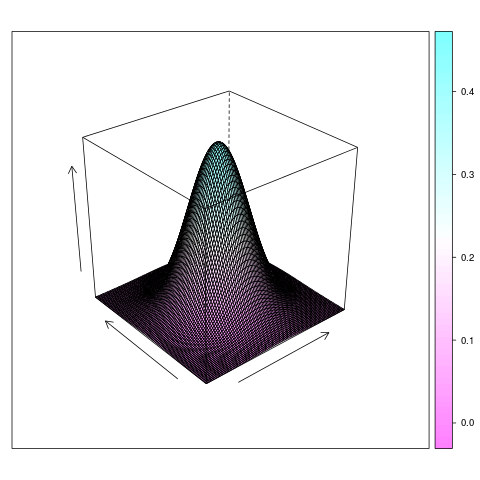
\includegraphics[width=.4\textwidth]{\fignet/FigRSyst-LPM-density}   
    & &
    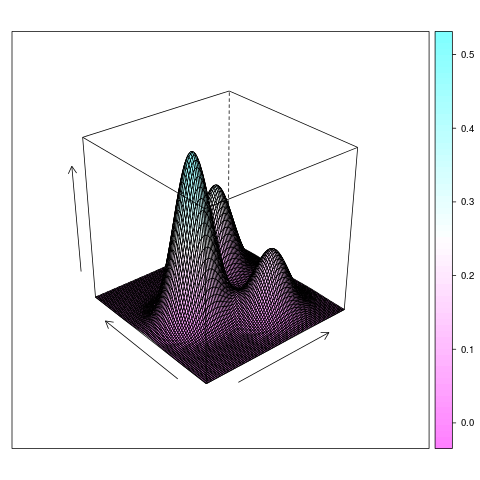
\includegraphics[width=.4\textwidth]{\fignet/FigRSyst-LPCM-density} \\       
  \end{tabular}
  \onslide<2>
  \begin{tabular}{ccc}
    unclustered model & & clustered model \\
    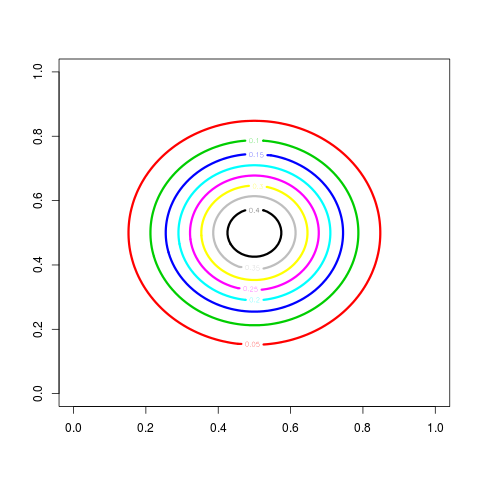
\includegraphics[width=.4\textwidth]{\fignet/FigRSyst-LPM-contour}   
    & &
    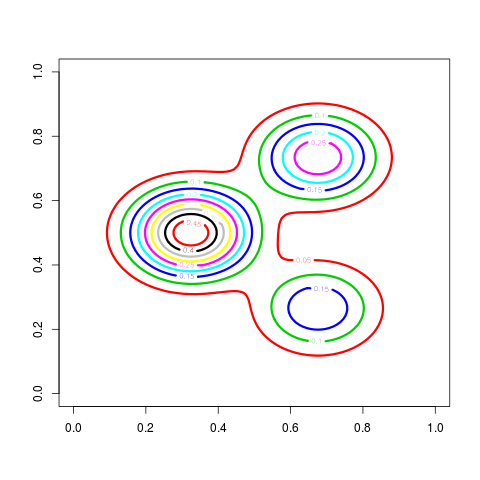
\includegraphics[width=.4\textwidth]{\fignet/FigRSyst-LPCM-contour} \\       
  \end{tabular}
  \end{overprint}
  $$
  
  
  }

%--------------------------------------------------------------------
\frame{\frametitle{A definition of clustering}

  \begin{tabular}{cc}
    \hspace{-.5cm}
    \begin{tabular}{p{.45\textwidth}}
    \paragraph{Definition.} A distribution $f$ is not clustered \emphase{at level $t$} if the set of points (level set)
    $$
    \Lcal(t) = \{z: f(z) > t\}
    $$
    is connected.
    
    \bigskip
    If not, denote $C(t)$ the number of connected sets.
    \end{tabular}
    & 
    \hspace{-.5cm}
    \begin{tabular}{p{.5\textwidth}}
    \begin{overprint}
	 \onslide<1>
	 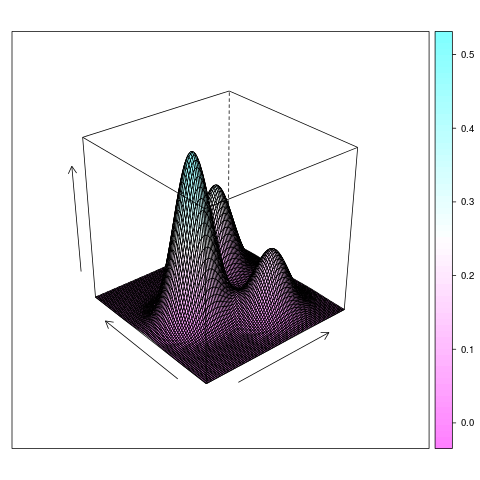
\includegraphics[width=.5\textwidth]{\fignet/FigRSyst-LPCM-density} 
	 \onslide<2>
	 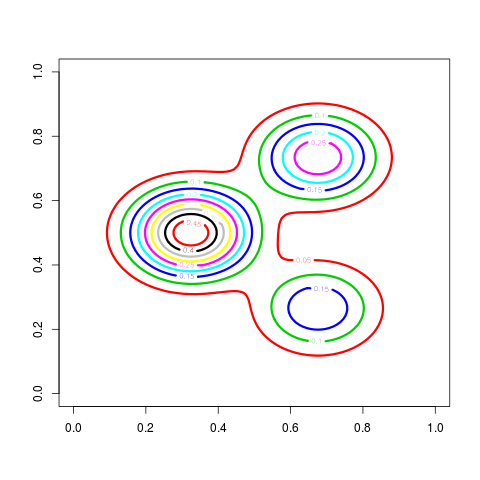
\includegraphics[width=.5\textwidth]{\fignet/FigRSyst-LPCM-contour} 
    \end{overprint}

    \end{tabular}
  \end{tabular}
  

}

%--------------------------------------------------------------------
\frame{\frametitle{A general model}

  \paragraph{Latent space.} Node positions $Z_i$ are distributed accord to $f$ (arbitrary and unknown).
  
  \bigskip \pause
  \paragraph{Connexion.} Node are connected with probability depending on their distance in the latent space:
  $$
  \Pr\{i \sim j | Z_i, Z_j\} = \gamma\left({\|Z_i - Z_j\|}/{h_n}\right)
  $$
  For identifiability reasons, one may assume that
  $
  \int \gamma(u) \dd u = 1.
  $
  
  \bigskip \pause
  \paragraph{Density estimation.} The normalized degree of a node provides an estimate of the density:
  $$
  T_i = \frac1{n-1} \sum_j Y_{ij}, \qquad
  \Esp(T_i | Z_i) = \frac1{n-1} \sum_j \gamma\left(\frac{\|Z_i - Z_j\|}{h_n}\right) \propto \widehat{f}(Z_i)
  $$
}

%--------------------------------------------------------------------
\subsection{A simple algorithm}
%--------------------------------------------------------------------
\frame{\frametitle{A simple algorithm}

  \begin{tabular}{cc}
    \hspace{-.5cm}
    \begin{tabular}{p{.5\textwidth}}
	 \begin{enumerate}
	 \onslide+<1->{\item Consider the whole graph $Y$ \\~}
	 \onslide+<2->{\item Select node with $T_i > t$ \\
	   \ra get an estimate $\widehat{\Lcal}(t)$ of $\Lcal(t)$ \\~}
	 \onslide+<3->{\item Count the number of connected components in the reduces graph \\
	   \ra get an estimate $\widehat{C}[\widehat{\Lcal}(t)]$ of $C(t)$}
	 \end{enumerate}
    \end{tabular}
    & 
    \hspace{-.5cm}
    \begin{tabular}{p{.5\textwidth}}
	 \begin{overprint}
	  \onslide<1>
	  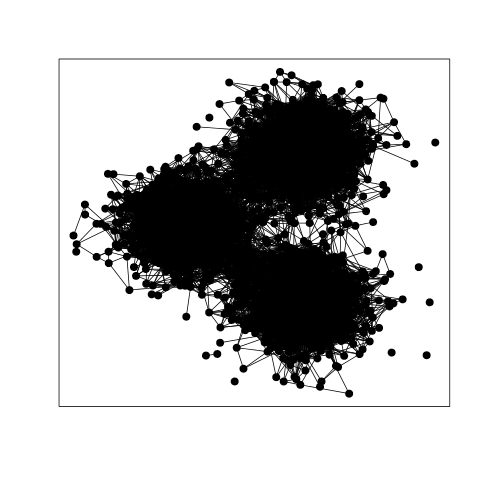
\includegraphics[width=.5\textwidth]{\fignet/FigRSyst-KerNet-K3}
	  \onslide<2-3>
	  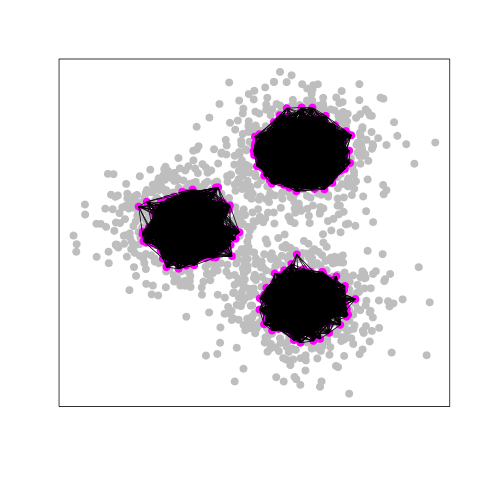
\includegraphics[width=.5\textwidth]{\fignet/FigRSyst-KerNet-K3-t36}
	 \end{overprint}
    \end{tabular}
  \end{tabular}

}

%--------------------------------------------------------------------
\subsection{Consistency}
%--------------------------------------------------------------------
\frame{\frametitle{Some theoretical results}

  Under standard (and nice) assumptions: 
  $$
  \begin{tabular}{lll}
  Non under-estimation:
  & &
  $\Pr\left\{\widehat{C}[\widehat{\Lcal}(t)] < C(t) \right\} \approx \lambda_1 n e^{-\kappa_1 n}$
  \\ ~\\
  Non over-estimation\footnote{beside density estimation error}:
  & &
  $\Pr\left\{\widehat{C}[{\Lcal}(t)] > C(t) \right\} \approx \lambda_2 n e^{-\kappa_2 n}$
  \\ ~\\
  All types of classification error:
  & &
  $\approx \lambda e^{-\kappa n}$
  \end{tabular}
  $$
  
  \bigskip
  \begin{itemize}
   \item \refer{BCP07} use the same algorithm (and prove similar results) to estimate the number of clusters when the position $Z_i$ are observed.
   \item \emphase{Channarond}'s results suggest that all relevant information is contained in the the degrees $T_i$.
  \end{itemize}


}


%--------------------------------------------------------------------
\subsection{Examples}
%--------------------------------------------------------------------
\frame{\frametitle{An example}

  \begin{tabular}{c}
    \hspace{.1\textwidth}
    \begin{overprint}
    \onslide<1>
    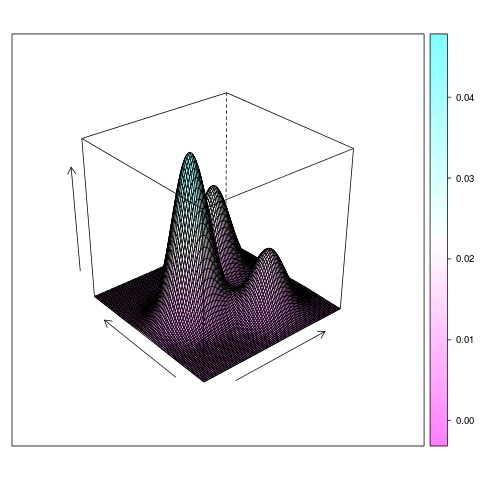
\includegraphics[width=.6\textwidth]{\fignet/FigRSyst-KerNet-K3-density}
    \onslide<2>
    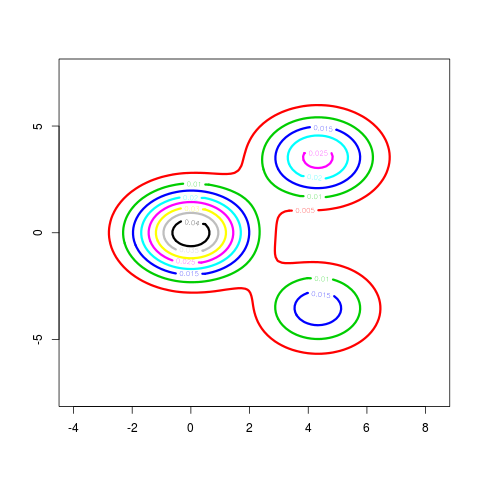
\includegraphics[width=.6\textwidth]{\fignet/FigRSyst-KerNet-K3-contour}    
    \onslide<3>
    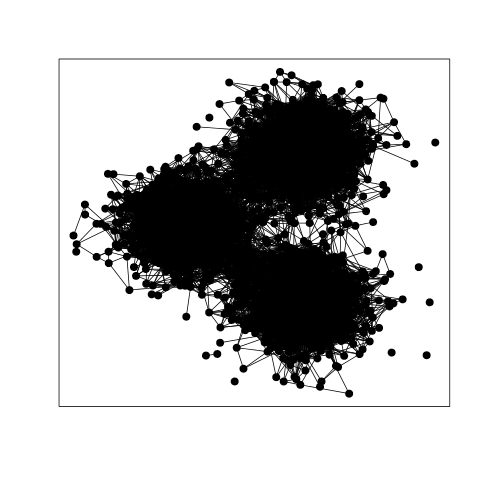
\includegraphics[width=.6\textwidth]{\fignet/FigRSyst-KerNet-K3}
    \onslide<4>
    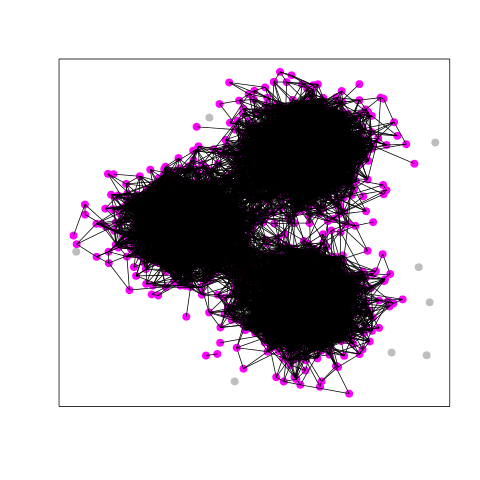
\includegraphics[width=.6\textwidth]{\fignet/FigRSyst-KerNet-K3-t2}
    \onslide<5>
    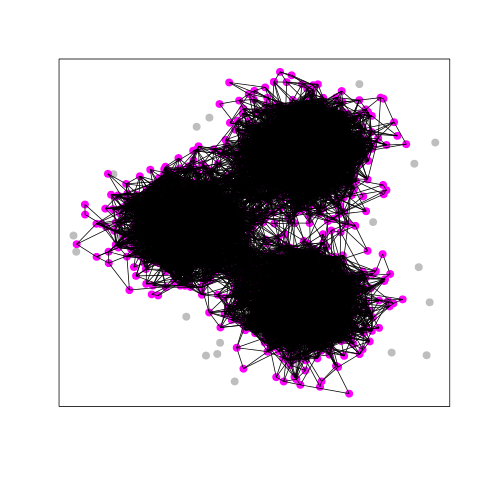
\includegraphics[width=.6\textwidth]{\fignet/FigRSyst-KerNet-K3-t3}
    \onslide<6>
    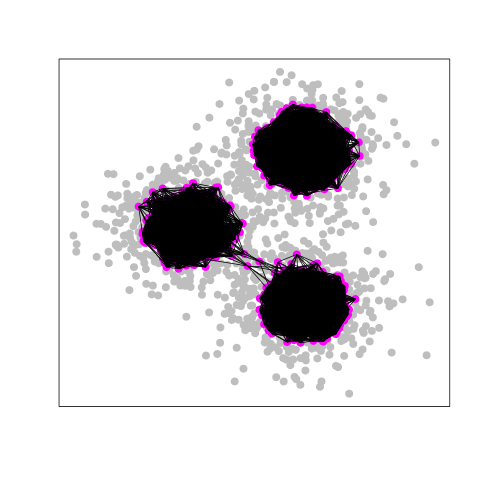
\includegraphics[width=.6\textwidth]{\fignet/FigRSyst-KerNet-K3-t33}
    \onslide<7>
    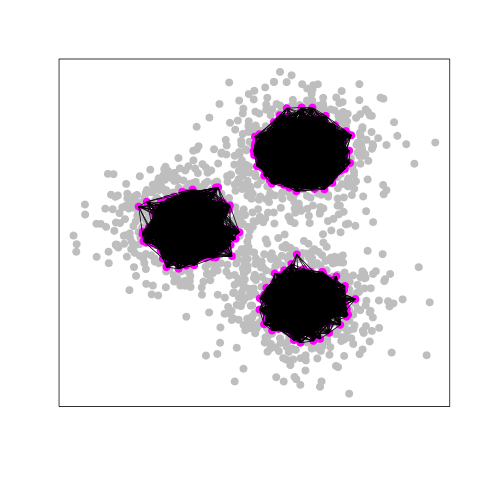
\includegraphics[width=.6\textwidth]{\fignet/FigRSyst-KerNet-K3-t36}
    \onslide<8>
    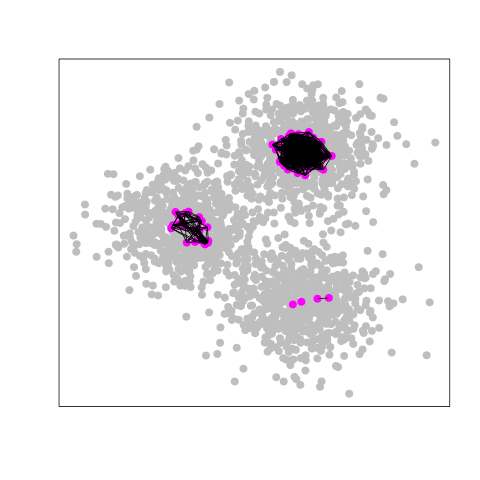
\includegraphics[width=.6\textwidth]{\fignet/FigRSyst-KerNet-K3-t68}
    \onslide<9>
    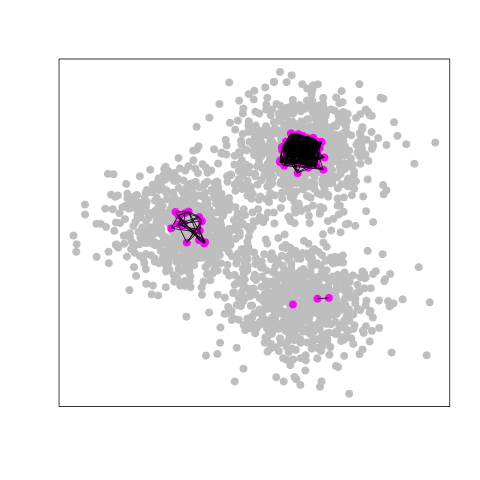
\includegraphics[width=.6\textwidth]{\fignet/FigRSyst-KerNet-K3-t70}
    \onslide<10>
    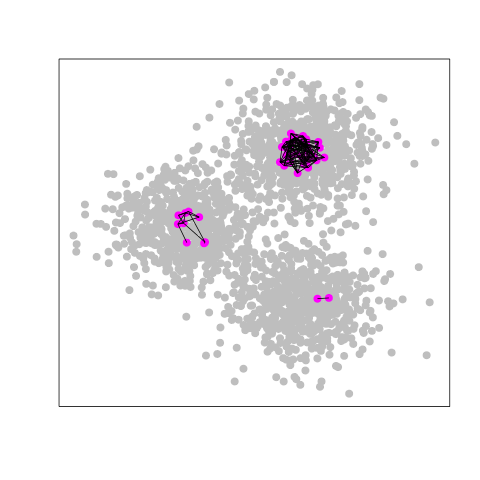
\includegraphics[width=.6\textwidth]{\fignet/FigRSyst-KerNet-K3-t72}
    \onslide<11>
    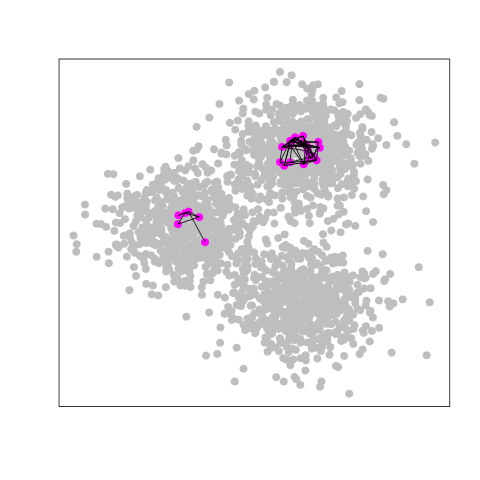
\includegraphics[width=.6\textwidth]{\fignet/FigRSyst-KerNet-K3-t74}
    \onslide<12>
    \hspace{-.18\textwidth}
    \begin{tabular}{ll}
    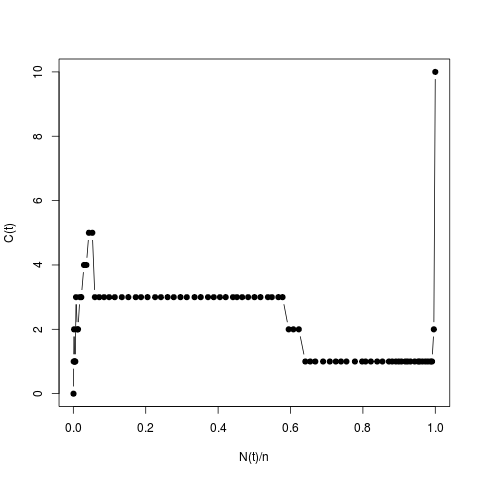
\includegraphics[width=.5\textwidth]{\fignet/FigRSyst-KerNet-K3-C-N}
    &
    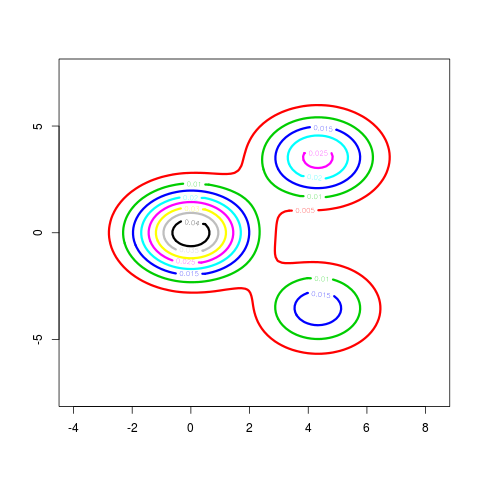
\includegraphics[width=.5\textwidth]{\fignet/FigRSyst-KerNet-K3-contour} \\
    $N(t) =$ nb nodes: $T_i \geq t$ & \multicolumn{1}{c}{True density contour} \\
    $C(t) =$ nb estimated clusters at level $t$ & 
    \end{tabular}
    \end{overprint}
  \end{tabular}

    
}

%--------------------------------------------------------------------
\frame{\frametitle{Another example}

  \begin{tabular}{c}
    \hspace{.1\textwidth}
    \begin{overprint}
    \onslide<1>
    \hspace{-.18\textwidth}
    \begin{tabular}{ll}
    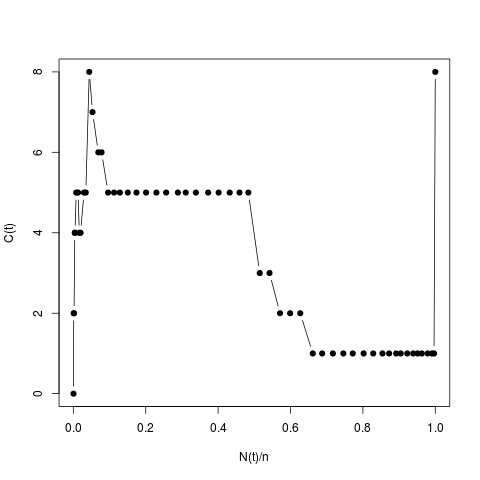
\includegraphics[width=.5\textwidth, clip=]{\fignet/FigRSyst-KerNet-K5-C-N}
    &
    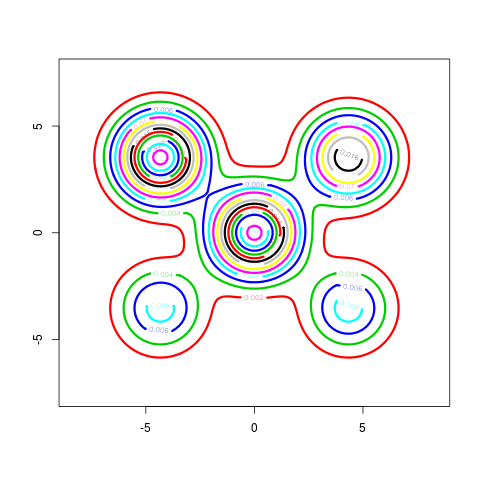
\includegraphics[width=.5\textwidth, clip=]{\fignet/FigRSyst-KerNet-K5-contour} \\    
    $N(t) =$ nb nodes: $T_i \geq t$ & \multicolumn{1}{c}{True density contour} \\
    $C(t) =$ nb estimated clusters at level $t$ & 
    \end{tabular}
    \end{overprint}
  \end{tabular}
    
}

%--------------------------------------------------------------------
{\tiny
  \bibliography{/home/robin/Biblio/ARC,/home/robin/Biblio/AST}%,/home/robin/Biblio/SSB}
  \bibliographystyle{/home/robin/LATEX/astats}
  %\bibliographystyle{plaine}
  }

%--------------------------------------------------------------------
%--------------------------------------------------------------------
\end{document}
%--------------------------------------------------------------------
%--------------------------------------------------------------------

  \begin{tabular}{cc}
    \hspace{-.5cm}
    \begin{tabular}{p{.5\textwidth}}
    \end{tabular}
    & 
    \hspace{-.5cm}
    \begin{tabular}{p{.5\textwidth}}
    \end{tabular}
  \end{tabular}

